% Options for packages loaded elsewhere
\PassOptionsToPackage{unicode}{hyperref}
\PassOptionsToPackage{hyphens}{url}
%
\documentclass[
  a4paper,
]{article}
\usepackage{amsmath,amssymb}
\usepackage{iftex}
\ifPDFTeX
  \usepackage[T1]{fontenc}
  \usepackage[utf8]{inputenc}
  \usepackage{textcomp} % provide euro and other symbols
\else % if luatex or xetex
  \usepackage{unicode-math} % this also loads fontspec
  \defaultfontfeatures{Scale=MatchLowercase}
  \defaultfontfeatures[\rmfamily]{Ligatures=TeX,Scale=1}
\fi
\usepackage{lmodern}
\ifPDFTeX\else
  % xetex/luatex font selection
  \setmainfont[]{Helvetica}
\fi
% Use upquote if available, for straight quotes in verbatim environments
\IfFileExists{upquote.sty}{\usepackage{upquote}}{}
\IfFileExists{microtype.sty}{% use microtype if available
  \usepackage[]{microtype}
  \UseMicrotypeSet[protrusion]{basicmath} % disable protrusion for tt fonts
}{}
\makeatletter
\@ifundefined{KOMAClassName}{% if non-KOMA class
  \IfFileExists{parskip.sty}{%
    \usepackage{parskip}
  }{% else
    \setlength{\parindent}{0pt}
    \setlength{\parskip}{6pt plus 2pt minus 1pt}}
}{% if KOMA class
  \KOMAoptions{parskip=half}}
\makeatother
\usepackage{xcolor}
\usepackage[margin=0.75in]{geometry}
\usepackage{graphicx}
\makeatletter
\def\maxwidth{\ifdim\Gin@nat@width>\linewidth\linewidth\else\Gin@nat@width\fi}
\def\maxheight{\ifdim\Gin@nat@height>\textheight\textheight\else\Gin@nat@height\fi}
\makeatother
% Scale images if necessary, so that they will not overflow the page
% margins by default, and it is still possible to overwrite the defaults
% using explicit options in \includegraphics[width, height, ...]{}
\setkeys{Gin}{width=\maxwidth,height=\maxheight,keepaspectratio}
% Set default figure placement to htbp
\makeatletter
\def\fps@figure{htbp}
\makeatother
\setlength{\emergencystretch}{3em} % prevent overfull lines
\providecommand{\tightlist}{%
  \setlength{\itemsep}{0pt}\setlength{\parskip}{0pt}}
\setcounter{secnumdepth}{-\maxdimen} % remove section numbering
\usepackage{titling}
\pretitle{\begin{flushleft}}
\posttitle{\end{flushleft}}
\usepackage{booktabs}
\usepackage{longtable}
\usepackage{float}
\floatplacement{figure}{H}
\usepackage{colortbl}
\usepackage{pdflscape}
\usepackage{tabu}
\usepackage{makecell}
\usepackage{xcolor}
\usepackage{soul}
\usepackage{caption}
\usepackage[singlelinecheck=false]{caption}
\usepackage[font={small,bf}]{caption}
\usepackage{multirow}
\usepackage{array}
\usepackage{lscape}
\newcommand{\blandscape}{\begin{landscape}}
\newcommand{\elandscape}{\end{landscape}}
\usepackage{booktabs}
\usepackage{longtable}
\usepackage{array}
\usepackage{multirow}
\usepackage{wrapfig}
\usepackage{float}
\usepackage{colortbl}
\usepackage{pdflscape}
\usepackage{tabu}
\usepackage{threeparttable}
\usepackage{threeparttablex}
\usepackage[normalem]{ulem}
\usepackage{makecell}
\usepackage{xcolor}
\ifLuaTeX
  \usepackage{selnolig}  % disable illegal ligatures
\fi
\usepackage{bookmark}
\IfFileExists{xurl.sty}{\usepackage{xurl}}{} % add URL line breaks if available
\urlstyle{same}
\hypersetup{
  hidelinks,
  pdfcreator={LaTeX via pandoc}}

\title{\vspace{-1.5cm} \begin{LARGE} WGS Quality Control Report \end{LARGE}}
\author{}
\date{\vspace{-2.5em}}

\begin{document}
\maketitle

\normalsize Batch Name: 2024-07-08

\normalsize Experiment Name: 24ARS\_EMR\_NGO\_LGH4F

\fontsize{7}{8}
\selectfont
\captionsetup[table]{labelformat=empty}
\renewcommand{\arraystretch}{1.2}

\begin{longtable}[t]{>{\centering\arraybackslash}p{1cm}>{\centering\arraybackslash}p{2cm}>{\centering\arraybackslash}p{1.5cm}>{\centering\arraybackslash}p{5.25cm}>{\centering\arraybackslash}p{5.25cm}}
\toprule
\multicolumn{1}{>{\centering\arraybackslash}p{1cm}}{\cellcolor[HTML]{D4D4D4}{\textbf{Isolate No.}}} & \multicolumn{1}{>{\centering\arraybackslash}p{2cm}}{\cellcolor[HTML]{D4D4D4}{\textbf{Sample ID}}} & \multicolumn{1}{>{\centering\arraybackslash}p{1.5cm}}{\cellcolor[HTML]{D4D4D4}{\textbf{Description}}} & \multicolumn{1}{>{\centering\arraybackslash}p{5.25cm}}{\cellcolor[HTML]{D4D4D4}{\textbf{ARSRL}}} & \multicolumn{1}{>{\centering\arraybackslash}p{5.25cm}}{\cellcolor[HTML]{D4D4D4}{\textbf{WGS}}}\\
\midrule
\cellcolor[HTML]{FFA77F}{1} & \cellcolor[HTML]{FFA77F}{22ARS\_BGH0063} & \cellcolor[HTML]{FFA77F}{NGO2} & \cellcolor[HTML]{FFA77F}{Neisseria gonorrhoeae} & \cellcolor[HTML]{FFA77F}{Neisseria gonorrhoeae}\\
2 & 22ARS\_BGH0094 & NGO4 & Neisseria gonorrhoeae & \cellcolor{white}{Neisseria gonorrhoeae}\\
3 & 22ARS\_BGH0095 & NGO5 & Neisseria gonorrhoeae & \cellcolor{white}{Neisseria gonorrhoeae}\\
4 & 22ARS\_BGH0096 & NGO6 & Neisseria gonorrhoeae & \cellcolor{white}{Neisseria gonorrhoeae}\\
5 & 22ARS\_GMH0061 & NGO9 & Neisseria gonorrhoeae & \cellcolor{white}{Neisseria gonorrhoeae}\\
\addlinespace
6 & 22ARS\_JLM0026 & NGO13 & Neisseria gonorrhoeae & \cellcolor{white}{Neisseria gonorrhoeae}\\
7 & 22ARS\_JLM0059 & NGO14 & Neisseria gonorrhoeae & \cellcolor{white}{Neisseria gonorrhoeae}\\
8 & 22ARS\_SLH0062 & NGO17 & Neisseria gonorrhoeae & \cellcolor{white}{Neisseria gonorrhoeae}\\
9 & 24ARS\_BGH0058 & EMR169 & Enterococcus faecalis & \cellcolor{white}{Enterococcus faecalis}\\
10 & 24ARS\_BGH0059 & EMR170 & Enterococcus faecalis & \cellcolor{white}{Enterococcus faecalis}\\
\addlinespace
11 & 24ARS\_BGH0061 & EMR171 & Enterococcus faecalis & \cellcolor{white}{Enterococcus faecalis}\\
12 & 24ARS\_BGH0062 & EMR172 & Enterococcus faecalis & \cellcolor{white}{Enterococcus faecalis}\\
13 & 24ARS\_BGH0065 & NGO3 & Enterococcus faecium & \cellcolor{yellow}{Neisseria gonorrhoeae}\\
14 & 24ARS\_DMC0129 & EMR168 & Enterococcus faecalis & \cellcolor{white}{Enterococcus faecalis}\\
15 & 24ARS\_JLM0064 & EMR163 & Pseudomonas aeruginosa & \cellcolor{white}{Pseudomonas aeruginosa}\\
\addlinespace
16 & 24ARS\_JLM0065 & EMR164 & Acinetobacter baumannii & \cellcolor{white}{Acinetobacter baumannii}\\
17 & 24ARS\_NKI0031 & EMR167 & Enterococcus faecalis & \cellcolor{white}{Enterococcus faecalis}\\
\cellcolor[HTML]{FD7979}{18} & \cellcolor[HTML]{FD7979}{24ARS\_NKI0054} & \cellcolor[HTML]{FD7979}{EMR160} & \cellcolor[HTML]{FD7979}{Pseudomonas aeruginosa} & \cellcolor[HTML]{FD7979}{Pseudomonas aeruginosa}\\
19 & 24ARS\_NKI0055 & EMR161 & Pseudomonas aeruginosa & \cellcolor{white}{Pseudomonas aeruginosa}\\
20 & 24ARS\_SLH0060 & EMR165 & Klebsiella pneumoniae & \cellcolor{white}{Klebsiella pneumoniae}\\
\addlinespace
21 & 24ARS\_SLH0064 & EMR166 & Pseudomonas aeruginosa & \cellcolor{white}{Pseudomonas aeruginosa}\\
22 & 24ARS\_STU0026 & EMR162 & Pseudomonas aeruginosa & \cellcolor{white}{Pseudomonas aeruginosa}\\
\bottomrule
\end{longtable}

\tiny Legend: \begingroup\fontsize{4}{6}\selectfont

\begin{tabular}{|>{\centering\arraybackslash}p{1cm}|>{\centering\arraybackslash}p{1cm}|>{\centering\arraybackslash}p{1cm}|>{\centering\arraybackslash}p{3cm}|>{\centering\arraybackslash}p{2cm}|}

\cellcolor{white}{PASS} & \cellcolor[HTML]{FFA77F}{WARNING} & \cellcolor[HTML]{FD7979}{FAILURE} & \textcolor{blue}{EXCEEDS THRESHOLD METRIC/S} & \cellcolor{yellow}{NON-CONCORDANT}\\

\end{tabular}
\endgroup{}
\fontsize{7}{8}
\selectfont
\captionsetup[table]{labelformat=empty}
\renewcommand{\arraystretch}{1.2}

\(\\\)

\fontsize{7}{8}
\selectfont
\captionsetup[table]{labelformat=empty}
\renewcommand{\arraystretch}{1.2}

\begin{longtable}[t]{>{\centering\arraybackslash}p{1cm}>{\centering\arraybackslash}p{3cm}>{\centering\arraybackslash}p{2cm}>{\centering\arraybackslash}p{2cm}>{\centering\arraybackslash}p{2cm}>{\centering\arraybackslash}p{2cm}>{\centering\arraybackslash}p{2cm}}
\toprule
\multicolumn{1}{>{\centering\arraybackslash}p{1cm}}{\cellcolor[HTML]{D4D4D4}{\textbf{Isolate No.}}} & \multicolumn{1}{>{\centering\arraybackslash}p{3cm}}{\cellcolor[HTML]{D4D4D4}{\textbf{Sample ID}}} & \multicolumn{1}{>{\centering\arraybackslash}p{2cm}}{\cellcolor[HTML]{D4D4D4}{\textbf{Contamination}}} & \multicolumn{1}{>{\centering\arraybackslash}p{2cm}}{\cellcolor[HTML]{D4D4D4}{\textbf{Contigs}}} & \multicolumn{1}{>{\centering\arraybackslash}p{2cm}}{\cellcolor[HTML]{D4D4D4}{\textbf{GC Percent}}} & \multicolumn{1}{>{\centering\arraybackslash}p{2cm}}{\cellcolor[HTML]{D4D4D4}{\textbf{N50}}} & \multicolumn{1}{>{\centering\arraybackslash}p{2cm}}{\cellcolor[HTML]{D4D4D4}{\textbf{Total Length}}}\\
\midrule
\cellcolor[HTML]{FFA77F}{1} & \cellcolor[HTML]{FFA77F}{22ARS\_BGH0063} & \cellcolor[HTML]{FFA77F}{\textcolor{black}{0}} & \cellcolor[HTML]{FFA77F}{\textcolor{black}{95}} & \cellcolor[HTML]{FFA77F}{52.55} & \cellcolor[HTML]{FFA77F}{\textcolor{blue}{46851}} & \cellcolor[HTML]{FFA77F}{2106578}\\
2 & 22ARS\_BGH0094 & \textcolor{black}{0} & \textcolor{black}{84} & 52.52 & \textcolor{black}{59655} & 2119302\\
3 & 22ARS\_BGH0095 & \textcolor{black}{0} & \textcolor{black}{84} & 52.64 & \textcolor{black}{64281} & 2076243\\
4 & 22ARS\_BGH0096 & \textcolor{black}{0} & \textcolor{black}{90} & 52.65 & \textcolor{black}{56218} & 2068914\\
5 & 22ARS\_GMH0061 & \textcolor{black}{0} & \textcolor{black}{88} & 52.64 & \textcolor{black}{57477} & 2071250\\
\addlinespace
6 & 22ARS\_JLM0026 & \textcolor{black}{0} & \textcolor{black}{81} & 52.29 & \textcolor{black}{60563} & 2191682\\
7 & 22ARS\_JLM0059 & \textcolor{black}{0} & \textcolor{black}{88} & 52.50 & \textcolor{black}{55092} & 2123392\\
8 & 22ARS\_SLH0062 & \textcolor{black}{0} & \textcolor{black}{86} & 52.48 & \textcolor{black}{52810} & 2122070\\
9 & 24ARS\_BGH0058 & \textcolor{black}{0} & \textcolor{black}{64} & 37.32 & \textcolor{black}{137544} & 2951077\\
10 & 24ARS\_BGH0059 & \textcolor{black}{0} & \textcolor{black}{54} & 37.17 & \textcolor{black}{179691} & 3086115\\
\addlinespace
11 & 24ARS\_BGH0061 & \textcolor{black}{0} & \textcolor{black}{38} & 37.47 & \textcolor{black}{264080} & 2883694\\
12 & 24ARS\_BGH0062 & \textcolor{black}{0} & \textcolor{black}{51} & 37.21 & \textcolor{black}{274808} & 3041435\\
13 & 24ARS\_BGH0065 & \textcolor{black}{0} & \textcolor{black}{86} & 52.50 & \textcolor{black}{65863} & 2130382\\
14 & 24ARS\_DMC0129 & \textcolor{black}{0} & \textcolor{black}{31} & 37.29 & \textcolor{black}{375662} & 2965797\\
15 & 24ARS\_JLM0064 & \textcolor{black}{0} & \textcolor{black}{58} & 66.03 & \textcolor{black}{310324} & 6603012\\
\addlinespace
16 & 24ARS\_JLM0065 & \textcolor{black}{0} & \textcolor{black}{50} & 38.90 & \textcolor{black}{162339} & 3872906\\
17 & 24ARS\_NKI0031 & \textcolor{black}{0} & \textcolor{black}{27} & 37.38 & \textcolor{black}{289851} & 2848700\\
\cellcolor[HTML]{FD7979}{18} & \cellcolor[HTML]{FD7979}{24ARS\_NKI0054} & \cellcolor[HTML]{FD7979}{\textcolor{black}{0}} & \cellcolor[HTML]{FD7979}{\textcolor{blue}{1198}} & \cellcolor[HTML]{FD7979}{66.29} & \cellcolor[HTML]{FD7979}{\textcolor{blue}{8862}} & \cellcolor[HTML]{FD7979}{6107910}\\
19 & 24ARS\_NKI0055 & \textcolor{black}{0} & \textcolor{black}{170} & 66.09 & \textcolor{black}{149562} & 6818848\\
20 & 24ARS\_SLH0060 & \textcolor{black}{0} & \textcolor{black}{34} & 57.43 & \textcolor{black}{494997} & 5317731\\
\addlinespace
21 & 24ARS\_SLH0064 & \textcolor{black}{0} & \textcolor{black}{62} & 66.34 & \textcolor{black}{321922} & 6392717\\
22 & 24ARS\_STU0026 & \textcolor{black}{0} & \textcolor{black}{108} & 65.55 & \textcolor{black}{184226} & 6998537\\
\bottomrule
\end{longtable}

\tiny Legend: \begingroup\fontsize{4}{6}\selectfont

\begin{tabular}{|>{\centering\arraybackslash}p{1cm}|>{\centering\arraybackslash}p{1cm}|>{\centering\arraybackslash}p{1cm}|>{\centering\arraybackslash}p{2.5cm}|>{\centering\arraybackslash}p{8cm}|}

\cellcolor{white}{PASS} & \cellcolor[HTML]{FFA77F}{WARNING} & \cellcolor[HTML]{FD7979}{FAILURE} & \textcolor{blue}{EXCEEDS THRESHOLD METRIC/S} & *Isolates were tagged with warning due to uncertain results  of species identification using bactinspector or sequence identification levels.\\

\end{tabular}
\endgroup{}

\fontsize{7}{8}
\selectfont
\captionsetup[table]{labelformat=empty}
\renewcommand{\arraystretch}{1.2}

\begin{longtable}[l]{cccccc}
\toprule
\multicolumn{6}{l}{\textbf{List of samples above/below QC threshold metrics}} \\
\cmidrule(l{3pt}r{3pt}){1-6}
\cellcolor[HTML]{D4D4D4}{\textbf{Sample ID}} & \cellcolor[HTML]{D4D4D4}{\textbf{Result}} & \cellcolor[HTML]{D4D4D4}{\textbf{Contamination}} & \cellcolor[HTML]{D4D4D4}{\textbf{Contigs}} & \cellcolor[HTML]{D4D4D4}{\textbf{N50}} & \cellcolor[HTML]{D4D4D4}{\textbf{Total Length}}\\
\midrule
24ARS\_NKI0054 & FAILURE & PASS & 1198 & 8862 & 6107910\\
\bottomrule
\end{longtable}

\fontsize{7}{8}
\selectfont
\captionsetup[table]{labelformat=empty}
\renewcommand{\arraystretch}{1.2}

\begin{longtable}[l]{>{\raggedright\arraybackslash}p{8cm}c}
\toprule
\cellcolor[HTML]{D4D4D4}{\textbf{WGS\_ID}} & \cellcolor[HTML]{D4D4D4}{\textbf{Number}}\\
\midrule
Neisseria gonorrhoeae & 9\\
Enterococcus faecalis & 6\\
Pseudomonas aeruginosa & 5\\
Acinetobacter baumannii & 1\\
Klebsiella pneumoniae & 1\\
\bottomrule
\end{longtable}

\begin{itemize}
\item
  \(\color{red}5\) distinct species were identified among
  \(\color{red}22\) isolates.
\item
  \(\color{red}90.91\) \% (n=20) of the isolates passed the QC, while
  \(\color{red}4.55\) \% (n=1) were tagged with warning.
\item
  Concordance between ARSRL and WGS species report was
  \(\color{red}95.45\) \%. \(\\\)
\end{itemize}

\subsubsection{GRAPHS}\label{graphs}

\fontsize{7}{8}
\selectfont
\captionsetup[table]{labelformat=empty}
\renewcommand{\arraystretch}{1.2}

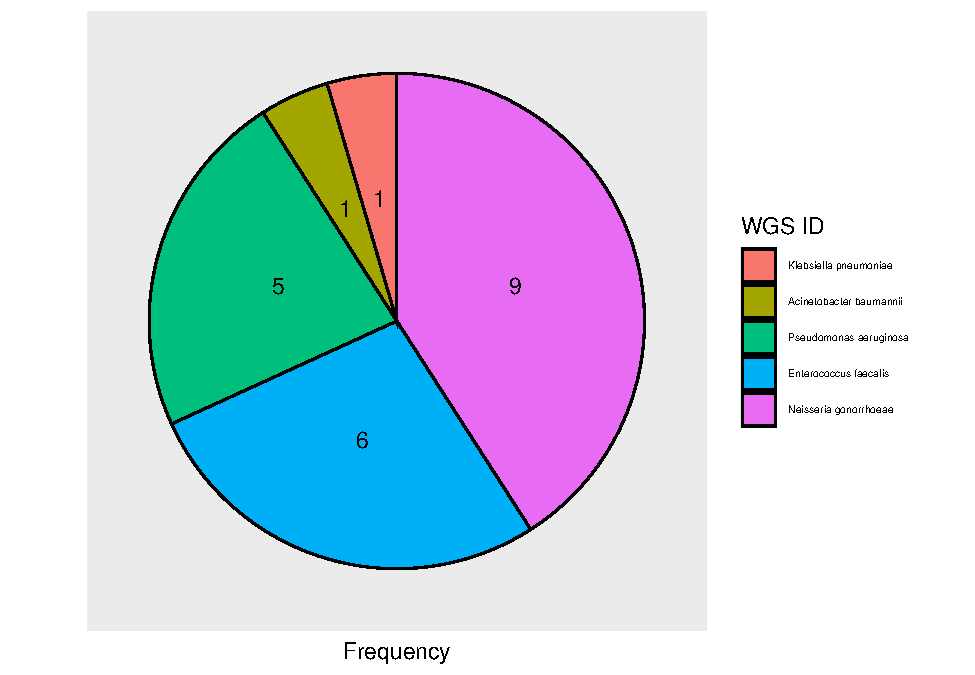
\includegraphics{qualifyr_report_2024-07-08_files/figure-latex/pie_chart-1.pdf}

\subsubsection{Result Classification}\label{result-classification}

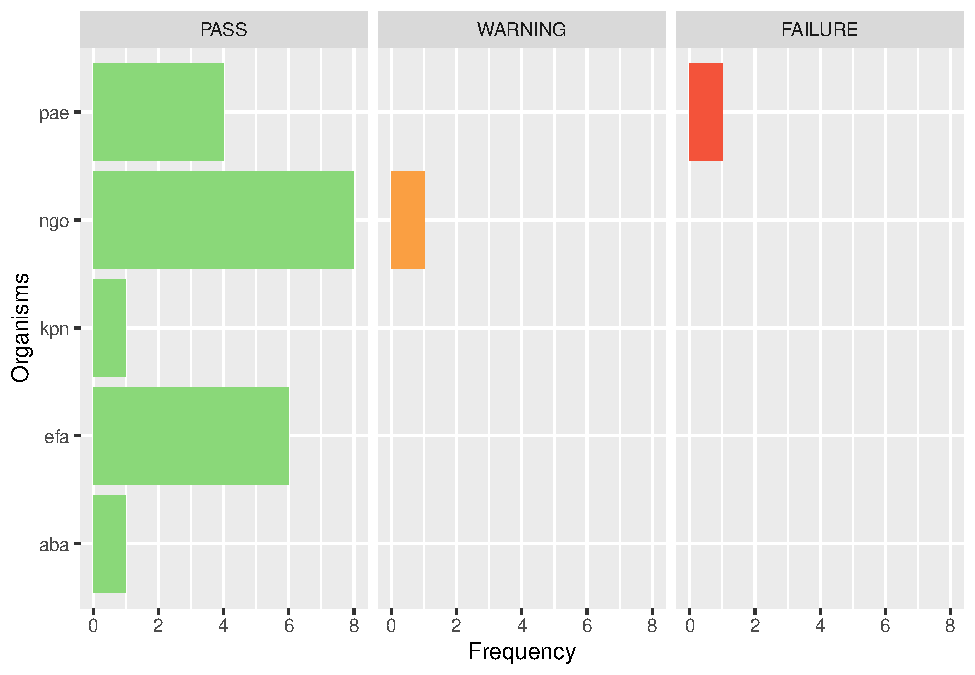
\includegraphics{qualifyr_report_2024-07-08_files/figure-latex/organism results-1.pdf}

\subsubsection{Number of contigs}\label{number-of-contigs}

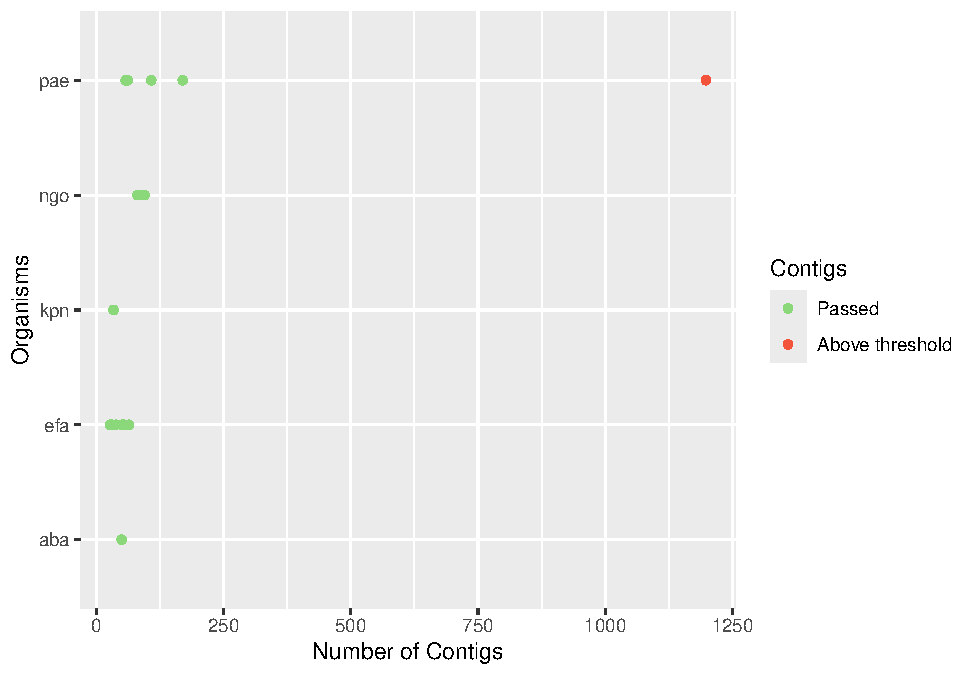
\includegraphics{qualifyr_report_2024-07-08_files/figure-latex/unnamed-chunk-1-1.pdf}

\subsubsection{N50 Value}\label{n50-value}

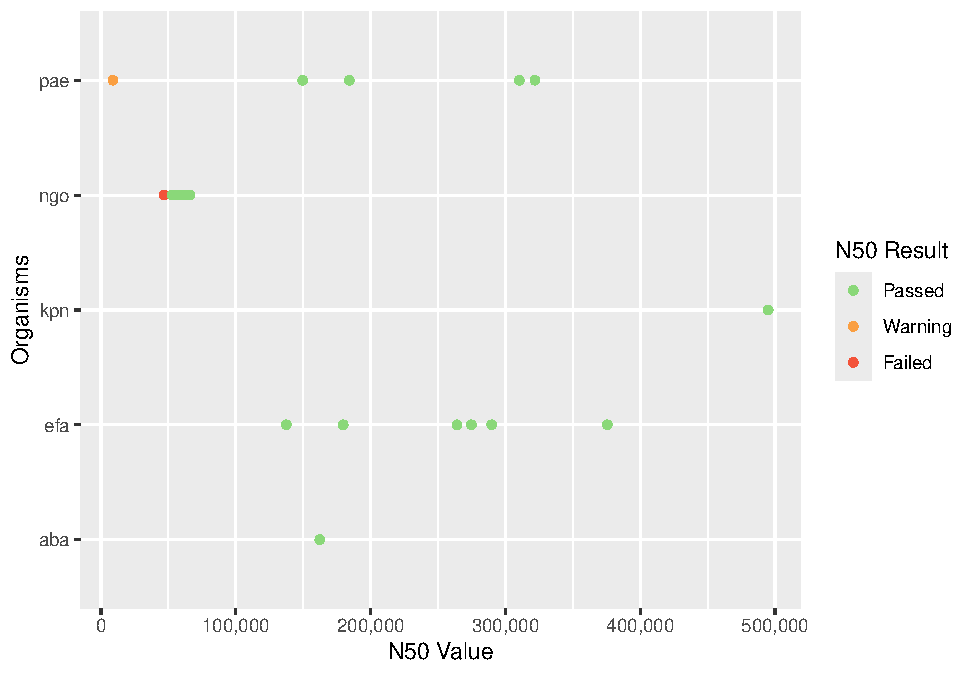
\includegraphics{qualifyr_report_2024-07-08_files/figure-latex/n50_result -1.pdf}

\subsubsection{Total Length}\label{total-length}

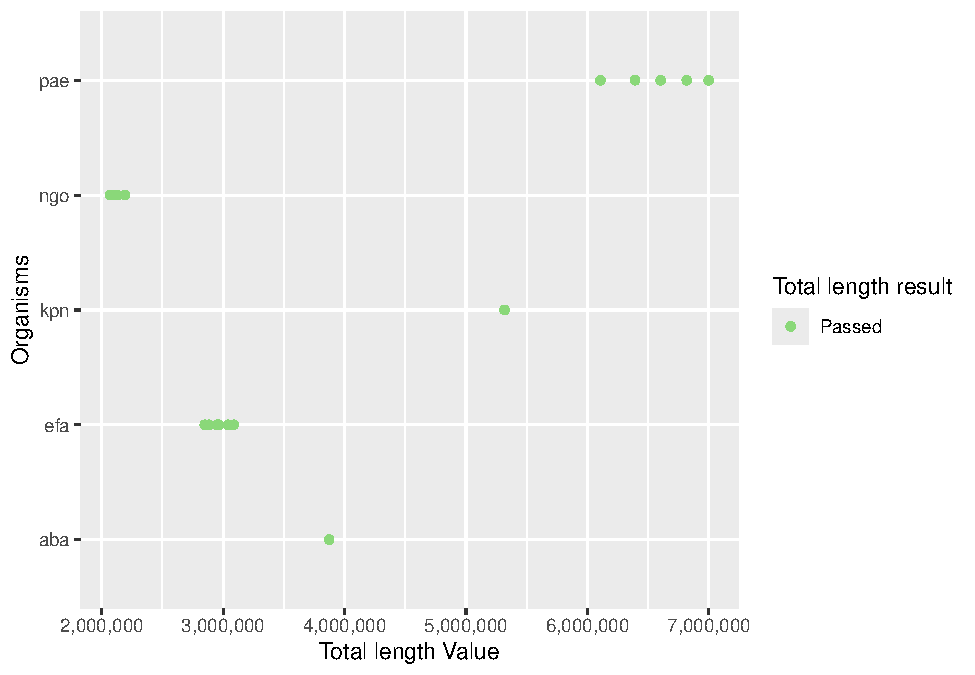
\includegraphics{qualifyr_report_2024-07-08_files/figure-latex/length_result -1.pdf}

\(\\\)

\subsubsection{RECOMMENDATION:}\label{recommendation}

\begin{longtable}[l]{>{\centering\arraybackslash}p{8cm}>{\centering\arraybackslash}p{3cm}>{\centering\arraybackslash}p{4cm}}
\toprule
\cellcolor[HTML]{D4D4D4}{\textbf{Sample ID}} & \cellcolor[HTML]{D4D4D4}{\textbf{Action}} & \cellcolor[HTML]{D4D4D4}{\textbf{Reason}}\\
\midrule
No further action required for this batch. &  & \\
\bottomrule
\end{longtable}

\subsubsection{MLST RESULTS}\label{mlst-results}

\begin{longtable}[l]{>{\centering\arraybackslash}p{3cm}>{\centering\arraybackslash}p{3cm}>{\centering\arraybackslash}p{1cm}>{\centering\arraybackslash}p{1cm}>{\centering\arraybackslash}p{1cm}>{\centering\arraybackslash}p{1cm}>{\centering\arraybackslash}p{1cm}>{\centering\arraybackslash}p{1cm}>{\centering\arraybackslash}p{1cm}c}
\toprule
\cellcolor[HTML]{D4D4D4}{\textbf{sample\_id}} & \cellcolor[HTML]{D4D4D4}{\textbf{species}} & \cellcolor[HTML]{D4D4D4}{\textbf{MLST}} & \cellcolor[HTML]{D4D4D4}{\textbf{abcZ}} & \cellcolor[HTML]{D4D4D4}{\textbf{adk}} & \cellcolor[HTML]{D4D4D4}{\textbf{aroE}} & \cellcolor[HTML]{D4D4D4}{\textbf{fumC}} & \cellcolor[HTML]{D4D4D4}{\textbf{gdh}} & \cellcolor[HTML]{D4D4D4}{\textbf{pdhC}} & \cellcolor[HTML]{D4D4D4}{\textbf{pgm}}\\
\midrule
22ARS\_BGH0063 & Neisseria gonorrhoeae & 13333 & 59 & 39 & 170 & 78 & 148 & 153 & 133\\
22ARS\_BGH0094 & Neisseria gonorrhoeae & 12463 & 109 & 39 & 170 & 78 & 149 & 154 & 65\\
22ARS\_BGH0095 & Neisseria gonorrhoeae & 11421 & 126 & 39 & 67 & 158 & 149 & 71 & 65\\
22ARS\_BGH0096 & Neisseria gonorrhoeae & - & 59 & 39 & \textasciitilde{}789 & 111 & 148 & 71 & 65\\
22ARS\_GMH0061 & Neisseria gonorrhoeae & 11963 & 59 & 39 & 67 & 111 & 149 & 154 & 65\\
\addlinespace
22ARS\_JLM0026 & Neisseria gonorrhoeae & - & 59 & \textasciitilde{}39 & 67 & 78 & 148 & 153 & 65\\
22ARS\_JLM0059 & Neisseria gonorrhoeae & 7363 & 59 & 39 & 67 & 78 & 148 & 153 & 65\\
22ARS\_SLH0062 & Neisseria gonorrhoeae & 8130 & 59 & 39 & 170 & 78 & 149 & 154 & 65\\
24ARS\_BGH0065 & Neisseria gonorrhoeae & 7363 & 59 & 39 & 67 & 78 & 148 & 153 & 65\\
\bottomrule
\end{longtable}
\vspace{1em}
\begin{longtable}[l]{>{\centering\arraybackslash}p{3cm}>{\centering\arraybackslash}p{3cm}>{\centering\arraybackslash}p{1cm}>{\centering\arraybackslash}p{1cm}>{\centering\arraybackslash}p{1cm}>{\centering\arraybackslash}p{1cm}>{\centering\arraybackslash}p{1cm}>{\centering\arraybackslash}p{1cm}>{\centering\arraybackslash}p{1cm}c}
\toprule
\cellcolor[HTML]{D4D4D4}{\textbf{sample\_id}} & \cellcolor[HTML]{D4D4D4}{\textbf{species}} & \cellcolor[HTML]{D4D4D4}{\textbf{MLST}} & \cellcolor[HTML]{D4D4D4}{\textbf{abcZ}} & \cellcolor[HTML]{D4D4D4}{\textbf{adk}} & \cellcolor[HTML]{D4D4D4}{\textbf{aroE}} & \cellcolor[HTML]{D4D4D4}{\textbf{fumC}} & \cellcolor[HTML]{D4D4D4}{\textbf{gdh}} & \cellcolor[HTML]{D4D4D4}{\textbf{pdhC}} & \cellcolor[HTML]{D4D4D4}{\textbf{pgm}}\\
\midrule
24ARS\_BGH0058 & Enterococcus faecalis & 368 & 63 & 6 & 67 & 6 & 23 & 1 & 68\\
24ARS\_BGH0059 & Enterococcus faecalis & 403 & 11 & 5 & 4 & 16 & 11 & 13 & 10\\
24ARS\_BGH0062 & Enterococcus faecalis & 179 & 5 & 1 & 1 & 3 & 7 & 1 & 6\\
24ARS\_DMC0129 & Enterococcus faecalis & 16 & 5 & 1 & 1 & 3 & 7 & 7 & 6\\
24ARS\_NKI0031 & Enterococcus faecalis & 16 & 5 & 1 & 1 & 3 & 7 & 7 & 6\\
\bottomrule
\end{longtable}
\vspace{1em}
\begin{longtable}[l]{>{\centering\arraybackslash}p{3cm}>{\centering\arraybackslash}p{3cm}>{\centering\arraybackslash}p{1cm}>{\centering\arraybackslash}p{1cm}>{\centering\arraybackslash}p{1cm}>{\centering\arraybackslash}p{1cm}>{\centering\arraybackslash}p{1cm}>{\centering\arraybackslash}p{1cm}>{\centering\arraybackslash}p{1cm}c}
\toprule
\cellcolor[HTML]{D4D4D4}{\textbf{sample\_id}} & \cellcolor[HTML]{D4D4D4}{\textbf{species}} & \cellcolor[HTML]{D4D4D4}{\textbf{MLST}} & \cellcolor[HTML]{D4D4D4}{\textbf{abcZ}} & \cellcolor[HTML]{D4D4D4}{\textbf{adk}} & \cellcolor[HTML]{D4D4D4}{\textbf{aroE}} & \cellcolor[HTML]{D4D4D4}{\textbf{fumC}} & \cellcolor[HTML]{D4D4D4}{\textbf{gdh}} & \cellcolor[HTML]{D4D4D4}{\textbf{pdhC}} & \cellcolor[HTML]{D4D4D4}{\textbf{pgm}}\\
\midrule
24ARS\_JLM0064 & Pseudomonas aeruginosa & - & 28 & 20 & 11 & 11 & 4 & 4 & \textasciitilde{}219\\
24ARS\_NKI0054 & Pseudomonas aeruginosa & - & - & 5 & 11 & 354? & 3 & 15 & 1\\
24ARS\_NKI0055 & Pseudomonas aeruginosa & 235 & 38 & 11 & 3 & 13 & 1 & 2 & 4\\
24ARS\_SLH0064 & Pseudomonas aeruginosa & 244 & 17 & 5 & 12 & 3 & 14 & 4 & 7\\
24ARS\_STU0026 & Pseudomonas aeruginosa & 277 & 39 & 5 & 9 & 11 & 27 & 5 & 2\\
\bottomrule
\end{longtable}
\vspace{1em}
\begin{longtable}[l]{>{\centering\arraybackslash}p{3cm}>{\centering\arraybackslash}p{3cm}>{\centering\arraybackslash}p{1cm}>{\centering\arraybackslash}p{1cm}>{\centering\arraybackslash}p{1cm}>{\centering\arraybackslash}p{1cm}>{\centering\arraybackslash}p{1cm}>{\centering\arraybackslash}p{1cm}>{\centering\arraybackslash}p{1cm}c}
\toprule
\cellcolor[HTML]{D4D4D4}{\textbf{sample\_id}} & \cellcolor[HTML]{D4D4D4}{\textbf{species}} & \cellcolor[HTML]{D4D4D4}{\textbf{MLST}} & \cellcolor[HTML]{D4D4D4}{\textbf{abcZ}} & \cellcolor[HTML]{D4D4D4}{\textbf{adk}} & \cellcolor[HTML]{D4D4D4}{\textbf{aroE}} & \cellcolor[HTML]{D4D4D4}{\textbf{fumC}} & \cellcolor[HTML]{D4D4D4}{\textbf{gdh}} & \cellcolor[HTML]{D4D4D4}{\textbf{pdhC}} & \cellcolor[HTML]{D4D4D4}{\textbf{pgm}}\\
\midrule
24ARS\_JLM0065 & Acinetobacter baumannii & 2 & 2 & 2 & 2 & 2 & 2 & 2 & 2\\
\bottomrule
\end{longtable}
\vspace{1em}
\begin{longtable}[l]{>{\centering\arraybackslash}p{3cm}>{\centering\arraybackslash}p{3cm}>{\centering\arraybackslash}p{1cm}>{\centering\arraybackslash}p{1cm}>{\centering\arraybackslash}p{1cm}>{\centering\arraybackslash}p{1cm}>{\centering\arraybackslash}p{1cm}>{\centering\arraybackslash}p{1cm}>{\centering\arraybackslash}p{1cm}c}
\toprule
\cellcolor[HTML]{D4D4D4}{\textbf{sample\_id}} & \cellcolor[HTML]{D4D4D4}{\textbf{species}} & \cellcolor[HTML]{D4D4D4}{\textbf{MLST}} & \cellcolor[HTML]{D4D4D4}{\textbf{abcZ}} & \cellcolor[HTML]{D4D4D4}{\textbf{adk}} & \cellcolor[HTML]{D4D4D4}{\textbf{aroE}} & \cellcolor[HTML]{D4D4D4}{\textbf{fumC}} & \cellcolor[HTML]{D4D4D4}{\textbf{gdh}} & \cellcolor[HTML]{D4D4D4}{\textbf{pdhC}} & \cellcolor[HTML]{D4D4D4}{\textbf{pgm}}\\
\midrule
24ARS\_SLH0060 & Klebsiella pneumoniae & 327 & 2 & 1 & 1 & 1 & 10 & 1 & 19\\
\bottomrule
\end{longtable}
\vspace{1em}

\subsubsection{MLST RESULTS SUMMARY:}\label{mlst-results-summary}

\begin{longtable}[l]{ll}
\toprule
\cellcolor[HTML]{D4D4D4}{\textbf{Species}} & \cellcolor[HTML]{D4D4D4}{\textbf{MLST}}\\
\midrule
Neisseria gonorrhoeae & - (n= 2 ),11421 (n= 1 ),11963 (n= 1 ),12463 (n= 1 ),13333 (n= 1 ),7363 (n= 2 ),8130 (n= 1 )\\
Enterococcus faecalis & 16 (n= 2 ),179 (n= 1 ),368 (n= 1 ),403 (n= 1 )\\
Pseudomonas aeruginosa & - (n= 2 ),235 (n= 1 ),244 (n= 1 ),277 (n= 1 )\\
Acinetobacter baumannii & 2 (n= 1 )\\
Klebsiella pneumoniae & 327 (n= 1 )\\
\bottomrule
\end{longtable}

\newpage
\begin{landscape}

\subsubsection{AMR PREDICTION RESULTS}\label{amr-prediction-results}

\begin{table}[H]
\centering
\resizebox{\ifdim\width>\linewidth\linewidth\else\width\fi}{!}{
\begin{tabular}{c>{\centering\arraybackslash}p{3cm}>{\centering\arraybackslash}p{3cm}>{\centering\arraybackslash}p{3cm}>{\centering\arraybackslash}p{3cm}>{\centering\arraybackslash}p{3cm}}
\toprule
\cellcolor[HTML]{D4D4D4}{\textbf{sample\_id}} & \cellcolor[HTML]{D4D4D4}{\textbf{species}} & \cellcolor[HTML]{D4D4D4}{\textbf{AMR BETA-LACTAM}} & \cellcolor[HTML]{D4D4D4}{\textbf{AMR EFFLUX}} & \cellcolor[HTML]{D4D4D4}{\textbf{AMR TETRACYCLINE}} & \cellcolor[HTML]{D4D4D4}{\textbf{STRESS EFFLUX}}\\
\midrule
22ARS\_BGH0063 & Neisseria gonorrhoeae & blaTEM-135 & norM, mtrC, mtrR, mtrA, farB & NA & mtrF\\
22ARS\_BGH0094 & Neisseria gonorrhoeae & blaTEM-135 & norM, mtrC, mtrR, mtrA, farB & tet(M) & mtrF\\
22ARS\_BGH0095 & Neisseria gonorrhoeae & blaTEM-1 & norM, mtrC, mtrR, mtrA, farB & NA & mtrF\\
22ARS\_BGH0096 & Neisseria gonorrhoeae & blaTEM-1 & norM, mtrC, mtrR, mtrA, farB & NA & mtrF\\
22ARS\_GMH0061 & Neisseria gonorrhoeae & blaTEM-135 & norM, mtrC, mtrR, mtrA, farB & NA & mtrF\\
\addlinespace
22ARS\_JLM0026 & Neisseria gonorrhoeae & blaTEM-1 & norM, mtrC, mtrR, farB, mtrA & tet(M) & mtrF\\
22ARS\_JLM0059 & Neisseria gonorrhoeae & blaTEM-1 & norM, mtrC, mtrR, farB, mtrA & tet(M) & mtrF\\
22ARS\_SLH0062 & Neisseria gonorrhoeae & blaTEM-135 & norM, mtrC, mtrR, mtrA, farB & tet(M) & mtrF\\
24ARS\_BGH0065 & Neisseria gonorrhoeae & blaTEM & norM, mtrC, mtrR, farB, mtrA & tet(M) & mtrF\\
\bottomrule
\end{tabular}}
\end{table}
\vspace{1em}\begin{table}[H]
\centering
\resizebox{\ifdim\width>\linewidth\linewidth\else\width\fi}{!}{
\begin{tabular}{c>{\centering\arraybackslash}p{3cm}>{\centering\arraybackslash}p{3cm}>{\centering\arraybackslash}p{3cm}>{\centering\arraybackslash}p{3cm}>{\centering\arraybackslash}p{3cm}>{\centering\arraybackslash}p{3cm}>{\centering\arraybackslash}p{3cm}>{\centering\arraybackslash}p{3cm}>{\centering\arraybackslash}p{3cm}>{\centering\arraybackslash}p{3cm}>{\centering\arraybackslash}p{3cm}>{\centering\arraybackslash}p{3cm}>{\centering\arraybackslash}p{3cm}>{\centering\arraybackslash}p{3cm}>{\centering\arraybackslash}p{3cm}>{\centering\arraybackslash}p{3cm}>{\centering\arraybackslash}p{3cm}}
\toprule
\cellcolor[HTML]{D4D4D4}{\textbf{sample\_id}} & \cellcolor[HTML]{D4D4D4}{\textbf{species}} & \cellcolor[HTML]{D4D4D4}{\textbf{AMR AMIKACIN/ GENTAMICIN/ KANAMYCIN/ TOBRAMYCIN}} & \cellcolor[HTML]{D4D4D4}{\textbf{AMR AMIKACIN/ KANAMYCIN}} & \cellcolor[HTML]{D4D4D4}{\textbf{AMR AMINOGLYCOSIDE}} & \cellcolor[HTML]{D4D4D4}{\textbf{AMR CHLORAMPHENICOL}} & \cellcolor[HTML]{D4D4D4}{\textbf{AMR CHLORAMPHENICOL/ FLORFENICOL}} & \cellcolor[HTML]{D4D4D4}{\textbf{AMR CLINDAMYCIN/ ERYTHROMYCIN/ STREPTOGRAMIN B}} & \cellcolor[HTML]{D4D4D4}{\textbf{AMR FLORFENICOL/ OXAZOLIDINONE}} & \cellcolor[HTML]{D4D4D4}{\textbf{AMR LINCOSAMIDE}} & \cellcolor[HTML]{D4D4D4}{\textbf{AMR LINCOSAMIDE/ STREPTOGRAMIN}} & \cellcolor[HTML]{D4D4D4}{\textbf{AMR MADURAMICIN/ NARASIN/ SALINOMYCIN}} & \cellcolor[HTML]{D4D4D4}{\textbf{AMR SPECTINOMYCIN}} & \cellcolor[HTML]{D4D4D4}{\textbf{AMR STREPTOMYCIN}} & \cellcolor[HTML]{D4D4D4}{\textbf{AMR STREPTOTHRICIN}} & \cellcolor[HTML]{D4D4D4}{\textbf{AMR TETRACYCLINE}} & \cellcolor[HTML]{D4D4D4}{\textbf{AMR TRIMETHOPRIM}} & \cellcolor[HTML]{D4D4D4}{\textbf{STRESS COPPER}}\\
\midrule
24ARS\_BGH0058 & Enterococcus faecalis & NA & aph(3')-IIIa & NA & NA & NA & NA & NA & NA & lsa(A) & narB, narA & ant(9)-Ia & ant(6)-Ia & sat4 & tet(M), tet(L) & NA & NA\\
24ARS\_BGH0059 & Enterococcus faecalis & aac(6')-Ie/aph(2'')-Ia & NA & spw & NA & fexA & erm(B) & optrA & lnu(B) & lsa(A), lsa(E) & narB, narA & ant(9)-Ia & ant(6)-Ia & NA & tet(M), tet(L) & NA & tcrB\\
24ARS\_BGH0062 & Enterococcus faecalis & NA & NA & NA & catA & NA & erm(B) & NA & NA & lsa(A) & NA & NA & str & NA & tet(M) & dfrG & NA\\
24ARS\_DMC0129 & Enterococcus faecalis & aac(6')-Ie/aph(2'')-Ia & aph(3')-IIIa & spw & NA & fexA & erm(B) & optrA & lnu(B) & lsa(A), lsa(E) & NA & NA & ant(6)-Ia & sat4 & tet(M) & dfrG & NA\\
24ARS\_NKI0031 & Enterococcus faecalis & aac(6')-Ie/aph(2'')-Ia & aph(3')-IIIa & spw & NA & fexA & erm(B) & optrA & lnu(B) & lsa(A), lsa(E) & NA & ant(9)-Ia & ant(6)-Ia & sat4 & tet(M) & NA & NA\\
\bottomrule
\end{tabular}}
\end{table}
\vspace{1em}\begin{table}[H]
\centering
\resizebox{\ifdim\width>\linewidth\linewidth\else\width\fi}{!}{
\begin{tabular}{c>{\centering\arraybackslash}p{3cm}>{\centering\arraybackslash}p{3cm}>{\centering\arraybackslash}p{3cm}>{\centering\arraybackslash}p{3cm}>{\centering\arraybackslash}p{3cm}>{\centering\arraybackslash}p{3cm}>{\centering\arraybackslash}p{3cm}>{\centering\arraybackslash}p{3cm}>{\centering\arraybackslash}p{3cm}>{\centering\arraybackslash}p{3cm}>{\centering\arraybackslash}p{3cm}>{\centering\arraybackslash}p{3cm}}
\toprule
\cellcolor[HTML]{D4D4D4}{\textbf{sample\_id}} & \cellcolor[HTML]{D4D4D4}{\textbf{species}} & \cellcolor[HTML]{D4D4D4}{\textbf{AMR BETA-LACTAM}} & \cellcolor[HTML]{D4D4D4}{\textbf{AMR CARBAPENEM}} & \cellcolor[HTML]{D4D4D4}{\textbf{AMR CEPHALOSPORIN}} & \cellcolor[HTML]{D4D4D4}{\textbf{AMR CHLORAMPHENICOL}} & \cellcolor[HTML]{D4D4D4}{\textbf{AMR EFFLUX}} & \cellcolor[HTML]{D4D4D4}{\textbf{AMR FOSFOMYCIN}} & \cellcolor[HTML]{D4D4D4}{\textbf{AMR KANAMYCIN}} & \cellcolor[HTML]{D4D4D4}{\textbf{AMR SULFONAMIDE}} & \cellcolor[HTML]{D4D4D4}{\textbf{AMR TIGECYCLINE}} & \cellcolor[HTML]{D4D4D4}{\textbf{STRESS MERCURY}} & \cellcolor[HTML]{D4D4D4}{\textbf{STRESS ORGANOMERCURY}}\\
\midrule
24ARS\_JLM0064 & Pseudomonas aeruginosa & blaOXA-50 & NA & blaPDC-5 & catB7 & mexA, mexX, mexE & fosA & aph(3')-IIb & NA & NA & NA & NA\\
24ARS\_NKI0054 & Pseudomonas aeruginosa & blaOXA-396 & NA & NA & catB7 & mexA & fosA & aph(3')-IIb & NA & NA & NA & NA\\
24ARS\_NKI0055 & Pseudomonas aeruginosa & blaOXA-488 & blaIMP-26 & blaPDC-35, blaOXA-10 & catB7 & mexA, mexX, mexE & fosA & aph(3')-IIb & sul1 & tmexC3, tmexD3, toprJ1 & merR, merT, merP & merC\\
24ARS\_SLH0064 & Pseudomonas aeruginosa & blaOXA-847 & NA & blaPDC-1 & catB7 & mexE, mexA, mexX & fosA & aph(3')-IIb & NA & NA & NA & NA\\
24ARS\_STU0026 & Pseudomonas aeruginosa & blaOXA & NA & blaPDC-5 & catB7 & mexA, mexE, mexX & fosA & aph(3')-IIb & NA & NA & NA & NA\\
\bottomrule
\end{tabular}}
\end{table}
\vspace{1em}\begin{table}[H]
\centering
\resizebox{\ifdim\width>\linewidth\linewidth\else\width\fi}{!}{
\begin{tabular}{c>{\centering\arraybackslash}p{3cm}>{\centering\arraybackslash}p{3cm}>{\centering\arraybackslash}p{3cm}>{\centering\arraybackslash}p{3cm}>{\centering\arraybackslash}p{3cm}>{\centering\arraybackslash}p{3cm}>{\centering\arraybackslash}p{3cm}>{\centering\arraybackslash}p{3cm}>{\centering\arraybackslash}p{3cm}>{\centering\arraybackslash}p{3cm}>{\centering\arraybackslash}p{3cm}>{\centering\arraybackslash}p{3cm}}
\toprule
\cellcolor[HTML]{D4D4D4}{\textbf{sample\_id}} & \cellcolor[HTML]{D4D4D4}{\textbf{species}} & \cellcolor[HTML]{D4D4D4}{\textbf{AMR AZITHROMYCIN/ ERYTHROMYCIN/ STREPTOGRAMIN}} & \cellcolor[HTML]{D4D4D4}{\textbf{AMR CARBAPENEM}} & \cellcolor[HTML]{D4D4D4}{\textbf{AMR CEPHALOSPORIN}} & \cellcolor[HTML]{D4D4D4}{\textbf{AMR EFFLUX}} & \cellcolor[HTML]{D4D4D4}{\textbf{AMR ERYTHROMYCIN}} & \cellcolor[HTML]{D4D4D4}{\textbf{AMR FOSFOMYCIN}} & \cellcolor[HTML]{D4D4D4}{\textbf{AMR GENTAMICIN}} & \cellcolor[HTML]{D4D4D4}{\textbf{AMR SPECTINOMYCIN/ STREPTOMYCIN}} & \cellcolor[HTML]{D4D4D4}{\textbf{AMR STREPTOMYCIN}} & \cellcolor[HTML]{D4D4D4}{\textbf{AMR SULFONAMIDE}} & \cellcolor[HTML]{D4D4D4}{\textbf{STRESS NICKEL}}\\
\midrule
24ARS\_JLM0065 & Acinetobacter baumannii & msr(E) & blaOXA-66, blaOXA-23 & blaADC-73 & adeC, amvA & mph(E) & abaF & armA & ant(3'')-IIa & aph(3'')-Ib, aph(6)-Id & sul2 & nreB\\
\bottomrule
\end{tabular}}
\end{table}
\vspace{1em}\begin{table}[H]
\centering
\resizebox{\ifdim\width>\linewidth\linewidth\else\width\fi}{!}{
\begin{tabular}{c>{\centering\arraybackslash}p{3cm}>{\centering\arraybackslash}p{3cm}>{\centering\arraybackslash}p{3cm}>{\centering\arraybackslash}p{3cm}>{\centering\arraybackslash}p{3cm}>{\centering\arraybackslash}p{3cm}>{\centering\arraybackslash}p{3cm}>{\centering\arraybackslash}p{3cm}>{\centering\arraybackslash}p{3cm}>{\centering\arraybackslash}p{3cm}>{\centering\arraybackslash}p{3cm}>{\centering\arraybackslash}p{3cm}>{\centering\arraybackslash}p{3cm}>{\centering\arraybackslash}p{3cm}>{\centering\arraybackslash}p{3cm}>{\centering\arraybackslash}p{3cm}>{\centering\arraybackslash}p{3cm}>{\centering\arraybackslash}p{3cm}>{\centering\arraybackslash}p{3cm}>{\centering\arraybackslash}p{3cm}}
\toprule
\cellcolor[HTML]{D4D4D4}{\textbf{sample\_id}} & \cellcolor[HTML]{D4D4D4}{\textbf{species}} & \cellcolor[HTML]{D4D4D4}{\textbf{AMR AZITHROMYCIN/ ERYTHROMYCIN/ SPIRAMYCIN/ TELITHROMYCIN}} & \cellcolor[HTML]{D4D4D4}{\textbf{AMR BETA-LACTAM}} & \cellcolor[HTML]{D4D4D4}{\textbf{AMR BLEOMYCIN}} & \cellcolor[HTML]{D4D4D4}{\textbf{AMR CARBAPENEM}} & \cellcolor[HTML]{D4D4D4}{\textbf{AMR CEPHALOSPORIN}} & \cellcolor[HTML]{D4D4D4}{\textbf{AMR CHLORAMPHENICOL}} & \cellcolor[HTML]{D4D4D4}{\textbf{AMR CHLORAMPHENICOL/ FLORFENICOL}} & \cellcolor[HTML]{D4D4D4}{\textbf{AMR EFFLUX}} & \cellcolor[HTML]{D4D4D4}{\textbf{AMR FOSFOMYCIN}} & \cellcolor[HTML]{D4D4D4}{\textbf{AMR KANAMYCIN}} & \cellcolor[HTML]{D4D4D4}{\textbf{AMR PHENICOL/ QUINOLONE}} & \cellcolor[HTML]{D4D4D4}{\textbf{AMR QUINOLONE}} & \cellcolor[HTML]{D4D4D4}{\textbf{AMR RIFAMYCIN}} & \cellcolor[HTML]{D4D4D4}{\textbf{AMR STREPTOMYCIN}} & \cellcolor[HTML]{D4D4D4}{\textbf{AMR SULFONAMIDE}} & \cellcolor[HTML]{D4D4D4}{\textbf{STRESS MERCURY}} & \cellcolor[HTML]{D4D4D4}{\textbf{STRESS NA}} & \cellcolor[HTML]{D4D4D4}{\textbf{STRESS ORGANOMERCURY}} & \cellcolor[HTML]{D4D4D4}{\textbf{STRESS QUATERNARY AMMONIUM}}\\
\midrule
24ARS\_SLH0060 & Klebsiella pneumoniae & mph(A) & blaSHV-1 & ble & blaNDM-1 & blaDHA, blaOXA-10 & cmlA5 & floR & kdeA, emrD & fosA & aph(3')-Ia & oqxB25, oqxA & qnrS1 & arr-2 & aadA1 & sul2, sul1 & merT, merP & fieF & merC & qacE\\
\bottomrule
\end{tabular}}
\end{table}
\vspace{1em}

\end{landscape}

\end{document}
